\chapter{Introduction}
\section*{27 - Settembre}
\section{Product based}
In \textit{Project-based SE} there is loop which nowdays cripples software since its early stages of development.
This is due to mutable nature of \textbf{requirements}, which often change throughout time along the features implemented by the software.
\begin{center}
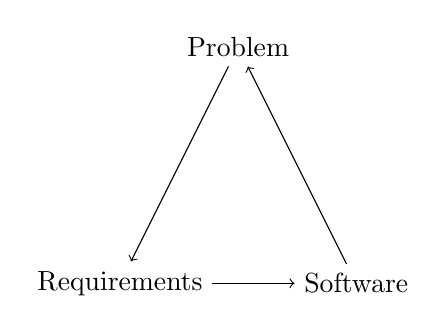
\begin{tikzpicture}
    \node[draw=white,align=left] (A) at (1.5,3) {Problem};
    \node[draw=white,align=left] (B) at (0,0) {Requirements};
    \node[draw=white,align=left] (C) at (3,0) {Software};

    \path [->] (A) edge node[left] {} (B);
    \path [->] (B) edge node[left] {} (C);    
    \path [->] (C) edge node[left] {} (A);    
\end{tikzpicture}
\end{center}

\textit{Product-based SE} is opposed to \textit{Project-based SE} and the above pictures changes as follows.

\begin{center}
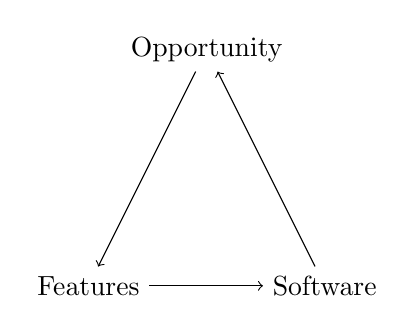
\begin{tikzpicture}
    \node[draw=white,align=left] (A) at (1.5,3) {Opportunity};
    \node[draw=white,align=left] (B) at (0,0) {Features};
    \node[draw=white,align=left] (C) at (3,0) {Software};

    \path [->] (A) edge node[left] {} (B);
    \path [->] (B) edge node[left] {} (C);    
    \path [->] (C) edge node[left] {} (A);    
\end{tikzpicture}
\end{center}

\section{Agile}
Agile is a collection of principles and methods applied in the software development field.
\nl

Opposed to project-based SE, in Agile the client is requested to express the requirements not in technical terms but in features.

Agile suggests an incremental development model

\subsection*{Principles}
\begin{enumerate}
    \label{subsec:agile_principles}
    \item \textbf{Satisfy} customer through early and \textbf{continuous delivery} of valuable software
    \item Welcome \textbf{changing requirement}, even late in development.
    Agile processes harness change for the customer's comptetitive advantage
    \item Deliver working software frequently, from a couple of weeks to a couple of months, with a preference to the \textbf{shorter timescale}
    \item Business people and devs must \textbf{work together} daily throughout the prokect
    \item Build projects around motivated \textbf{individuals} and give them the environment and support they need
    \item The most efficient and effective method of conveying information to and within a dev team is \textbf{face-to-face conversation}
    \item \textbf{Working software} is the primary measure of progress
    \item Agile processes promote sustainable development
    \item Continuous attention to technical excellence and good \textbf{design} enhances agility
    \item \textbf{Simplicity} i.e. art of maximizing the amount of work not done is essential
    \item The best architectures, requirements, and designs emerge from \textbf{self-organizing} teams.
\end{enumerate}

\textit{Extreme Programming} was proposed as part of the agile methodology.

\section{Scrum}
Since requirements changes are rather frequent, long-term plans are unreliable,
hence SE aims to formulate short-term plans.

Scrum is found on \textbf{empiricism} and \textbf{lean thinking}; it asserts that knowledge comes from experience, and that decisions should be made on observations.

Other key terms are code \textbf{Transparency} among the team and with the customer, \textbf{Inspection} of produced code and software (artifacts), \textbf{Adaptation} to changes in features and requirements.

The \textbf{Scrum Team} is composed by:
\begin{enumerate}
    \item \textbf{Product Owner}: must ensure that the dev team is always focused on the goal
    \item \textbf{Scrum Master}: Scrum expert which drives the team to apply properly the Scrum framework.
    \item \textbf{Developers}: actual \st{\textit{monkeys}} people which write code
\end{enumerate}

In scrum SW is developed in \textbf{sprints}, i.e. fixed-length periods with a specific goal to be achieved.

\begin{itemize}
    \item Product backlog: to-do list of items to be implemented
    \item Timeboxed sprints
    \item Self-organizing teams
\end{itemize}

\subsection{Product Backlog}
Key point of the scrum methodology,
it is a to-do list and its items are called \textbf{PBIs}\footnote{\textit{Product Backlog Item}}.
It is \textbf{prioritized},
so that the items that
be implemented first are at the top of the list

\labelitemize{
    \textit{Product Backlog Activities}
}{
    \begin{itemize}
        \item \textbf{Refinement}
        Existing PBIs are analysed and refined to create more detailed PBIs. This may
        lead to the creation of new product backlog items.
        \item \textbf{Estimation}
        The team estimate the amount of work required to implement a PBI and add this
        assessment to each analysed PBI.
        \item \textbf{Creation}
        New items are added to the backlog. These may be new features suggested by
        the product manager, required feature changes, engineering improvements, or
        process activities such as the assessment of development tools that might be
        used.
        \item \textbf{Prioritization}
        The product backlog items are reordered to take new information and changed
        circumstances into account.
    \end{itemize}
}


\subsection{Timeboxed Sprints}
Even if at the end of a srpint the goal hasn't been reached, "no worries", the work stops anyway;
there will be a new sprint which will include the work which has not been implemented in the previous one.

\subsection{Scrum Meetings}
During a sprint, the team has daily meetings (\textit{Scrums}) to \textbf{review} progress
and to update the list of work items that are incomplete.

\subsection{Agile suggested techniques}
\begin{itemize}
    \item \textbf{Test automation}
    As far as possible, product testing should be automated. You should
    develop a suite of executable tests that can be run at any time.
    \item \textbf{Continuous integration}
    Whenever anyone makes changes to the software components they are
    developing, these components should be immediately integrated with
    other components to create a system. This system should then be tested
    to check for unanticipated component interaction problems.
\end{itemize}

\subsection{Sprint reviews}
At the end of each sprint there is a review meeting which involves the \textit{whole} team.
The \textit{product owner} has the ultimate authority to decide wether the sprint goal has been reached or not.
The sprint review should include a process review, in which the whole team shares ideas on how to improve their way of working.

\begin{figure}[htbp]
    \centering
    \includegraphics[width=0.45\columnwidth]{images/scrum_cycles.png}
    \caption{Scrum cycles}
    \label{fig:scrum_cycles}
\end{figure}

